\usetikzlibrary{arrows.meta}
\begin{frame}{carrier sense}
    \begin{itemize}
    \item channel can be `busy' or not
    \item radio/light:
        \begin{itemize}
        \item have some sort of signal detectable on frequency
        \end{itemize}
    \vspace{.5cm}
    \item ``carrier sense''
    \item way to detect whether channel busy
    \end{itemize}
\end{frame}

\begin{frame}{using carrier sense}
    \begin{itemize}
    \item simple idea: don't transmit if channel already busy
    \vspace{.5cm}
    \item problem: then when do you transmit?
    \item some options:
        \begin{itemize}
        \item never, lose the packet
        \item immediately when it stops being busy
        \item sometime after it stops being busy
        \end{itemize}
    \end{itemize}
\end{frame}

\begin{frame}{`slots'}
\begin{itemize}
\item if packets take a fixed amount of time\ldots
\item want to wait whole number of packet times
    \begin{itemize}
    \item immediately after, one after, two after, three after
    \end{itemize}
\item avoids requiring almost 2 packets worth of `quiet' time
\item can synchronize by observing end of last transmission, or central clock
\end{itemize}
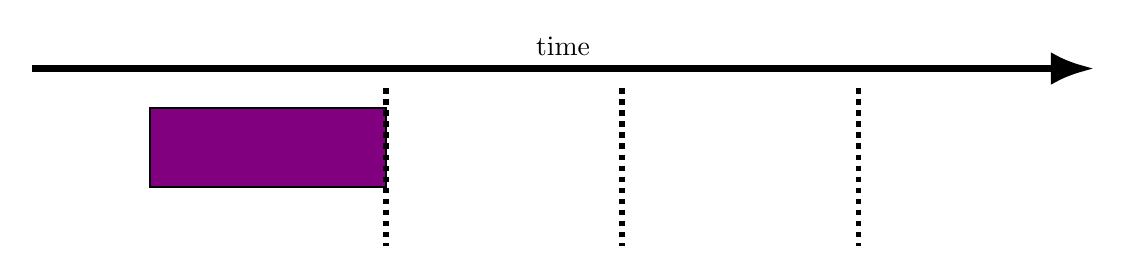
\begin{tikzpicture}
\begin{scope}[x=3cm]
    \draw[line width=1mm,-Latex] (-0.5, 0) -- (4, 0) node[above,midway] {time};
    \draw[thick,fill=violet] (0.0, -0.5) rectangle ++(1, -1);
    \foreach \x in {1,2,3} {
        \draw[dotted,line width=0.7mm] (\x, -0.25) -- ++ (0, -2);
    }
\end{scope}
\end{tikzpicture}
\end{frame}

\begin{frame}{fixed-size frames, slots}
    \begin{itemize}
    \item `slotted' Aloha
    \item challenge: synchronize everyone's timing
    \item then: everyone chooses slots to (re)transmit in
    \item but: not using carrier-sense before sending
        \begin{itemize}
        \item if everyone sync'd, not useful with fixed-size packets
        \end{itemize}
    \vspace{.5cm}
    \item requires 1-packet-unit empty periods
    \item 36\% utilization (twice for naive version)
    \end{itemize}
\end{frame}

\begin{frame}{802.11b typical slots}
    \begin{itemize}
    \item $20 \mu\text{s}$ slots
    \item $50 \mu\text{s}$ interframe spacing (IFS)
        \begin{itemize}
        \item includes time to receive ACK of packet
        \end{itemize}
    \vspace{.5cm}
    \item transmit first time after IFS (if idle)
    \item transmit second time after IFS + rand($0$, $2^5$) slots
        \begin{itemize}
        \item plus time spent by other seen transmissions
        \end{itemize}
    \item third time after rand($0$, $2^6$) slots, etc.
    \end{itemize}
\end{frame}

\begin{frame}{802.11b packet lengths}
    \begin{itemize}
    \item variable bit rate: max = 11Mbit
    \item approx 300--12000 bit frames
        \begin{itemize}
        \item = 27 to 1090 microseconds
        \end{itemize}
    \vspace{.5cm}
    \item do carrier sense before transmitting always
    \item different purpose for slots than slotted Aloha
    \end{itemize}
\end{frame}
